% This file is for the problem formulation section of the Master's Thesis.
% This file will not compile on it's own. Will need to include it into a main file
% That uses the drexel thesis template.
\chapter{Problem Formulation}

Detecting frame deletion in a video requires detecting the structural changes in a video due to the deletion process. In particular, Wang and Farid's work on temporal traces for detecting frame deletion shows that for MPEG-2 video, the P-frame prediction error can be formulated into a sequence. This sequence can then be monitored to detect frame deletion. Both Wang and Farid, and Stamm et al. use a system like in Fig.~\ref{System} to detect frame deletion. The prediction error sequence $e(n)$ is extracted from the decoded video file and processed to produce detection features. Wang and Farid's work did not propose features for automatic detection, and instead relied on visual inspection of the DFT of the prediction error sequence \cite{wang} \cite{stamm}.

\begin{figure}[htbp]
\centerline{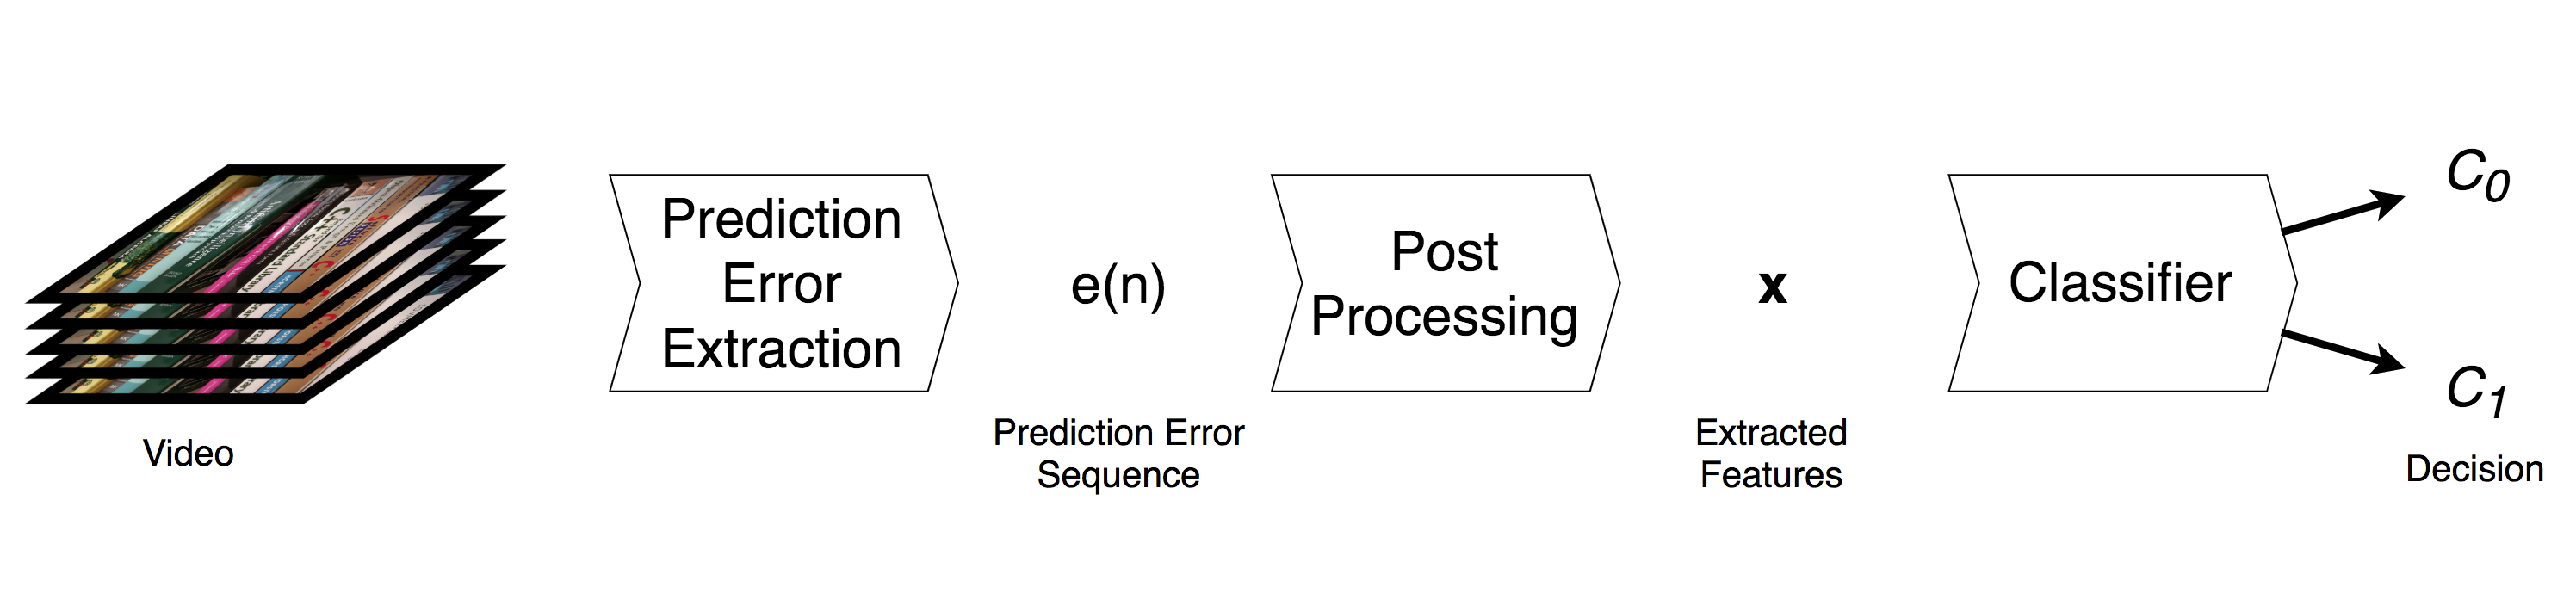
\includegraphics[width=0.9\linewidth]{ProblemFormulation/frame_deletion_detection_system.png}}
\caption{Generalized Approach to Frame Deletion Detection}
\label{System}
\end{figure}

This broad approach can also be applied to work with H.264 encoded video as well. While video encoding has advanced significantly, the fundamental structures of a compressed digital video have remained unchanged. Regardless of codec, the hallmark of video compression is the motion compensation and estimation process. Video frames are organized into GOPs that begin with an I-frame, and have varying structures of P and B-frames. In H.264, GOP structures are more dynamic due to the ability to derive motion-vector predictions from across multiple anchor frames. To remain robust to these advances in video compression, the prediction error extraction and post processing steps must be altered or augmented.

This work is concerned particularly with the detection of frame deletion in H.264 and similar modern video codecs. Frame addition has also been observed to introduce similar traces in the P-frame prediction error sequence as frame deletion. Our proposed system can be applied to detecting frame addition and for simplicity we will not discuss the detection of frame addition for the remainder of this thesis. We have made the following assumptions regarding our proposed system. First, we assume that all altered video has undergone re-compression. In fact, since most consumer video recording devices do not have the storage capability or processing power to record high-definition raw video, it is assumed that all video sources have been compressed by either MPEG-4 or H.264, and that all frame deleted video will be re-compressed using H.264 or a similar codec, where the reencoding is set to match the GOP structure of the source video. 

In addition, it is assumed that all videos that are passed to the detector are of sufficient length to make a classification. Without multiple full GOPs, the presence of a deletion fingerprint is negligible. Lastly, we make the assumption that if indeed frames have been removed from a video, they have not been removed from the end of the video. The detection features are dependent on differences between the structure of the prediction error sequences in natural videos versus videos with frame deletion. When frames are removed from the end of the video sequence, this difference is not observable. 

A user of our proposed system will not need physical access to a specific device to analyze a video captured by the device. The system should accept videos of an arbitrary length, and will not require metadata unrelated to video playback to be intact. It will work with videos of any resolution, frame rate, or GOP structure. Also, as our approach will be data driven, it is imperative that a user have access to a sufficient database of videos with known labels.

\section{Video Frame Deletion Detection}

Detecting frame deletion is a binary classification problem. Given a Video $V$, there are two possible classes:

\begin{equation}
\begin{aligned}
  C_{0} &: \text{The video is genuine, and has not had frames removed from it.} \\
  C_{1} &: \text{The video is altered, and has had frames removed from it.}
\end{aligned}
\end{equation}

Note that in this case, \emph{genuine} refers to the fact that the video has not undergone any additional post processing after its original capture. We will simply be considering the limited scenario whereby video has either come directly from the camera that captured it, or frames have been removed from the video and it has been recompressed. Any mention of a genuine video for the rest of this thesis refers to a video that has not been modified since it's original capture.

In general, it is difficult to classify whether or not a video has had frames removed based on the entirety of a video directly. Thus, the problem must be reworked. As shown above, a feature extraction system will be used to produce the P-frame prediction error sequence $e(n)$, and a feature vector $\bm{x}$. The feature vector ideally contains information about the prediction error sequence that can perfectly separate the two classes. As such, the classification problem is as follows. Given a feature vector $\bm{x}'$, it belongs to one of two classes:

\begin{equation}
\begin{aligned}
  C_{0} &: \bm{x}' \text{resulted from a genuine video that has not had frames removed from it.} \\
  C_{1} &: \bm{x}' \text{resulted from an altered video which has had frames removed from it.}
\end{aligned}
\end{equation}

In the following chapter, we will propose both a new method for extracting $e(n)$, and additional augmentations to $\bm{x}$ that allow for improved separation of data and increased robustness of the overall system.
